% =====================================================================
% ICONIP-style submission draft (Springer LNCS)
% Project: DimASQP-Refine
% Current result version: V16 / final per-dataset mix
% Build: pdflatex paper_iconip_current.tex
% =====================================================================
\documentclass[runningheads]{llncs}

\usepackage[T1]{fontenc}
\usepackage{graphicx}
\usepackage{amsmath,amssymb}
\usepackage{booktabs}
\usepackage{multirow}
\usepackage{url}
\usepackage{xcolor}
\usepackage{enumitem}
\usepackage{hyperref}
\hypersetup{
  pdftitle={LEADER-DimASQP: Language-Specific Encoder and Data-Aware Ensemble Refinement for Dimensional ASQP},
  pdfauthor={Hongzhen Qin, Yoshimi Suzuki, Fumiyo Fukumoto, Renjie Zhou},
  pdfkeywords={Aspect-Based Sentiment Analysis, Valence-Arousal, Multilingual NLP, Encoder Selection, Ensemble Learning}
}

\begin{document}

\title{\texorpdfstring{LEADER-DimASQP: Language-Specific Encoder and\\
Data-Aware Ensemble Refinement for Dimensional ASQP}{LEADER-DimASQP: Language-Specific Encoder and Data-Aware Ensemble Refinement for Dimensional ASQP}}
\titlerunning{LEADER-DimASQP}

\author{Hongzhen Qin\inst{1} \and Yoshimi Suzuki\inst{1} \and
Fumiyo Fukumoto\inst{1} \and Renjie Zhou\inst{2}}
\authorrunning{H.~Qin et al.}
\institute{University of Yamanashi, Kofu, Japan\\
\email{\{g24tka12,ysuzuki,fukumoto\}@yamanashi.ac.jp}
\and
School of Computer Science and Technology, Hangzhou Dianzi University,
Hangzhou 310018, China\\
\email{rjzhou@hdu.edu.cn}}

\maketitle

\begin{abstract}
Dimensional Aspect-Based Sentiment Analysis extends Aspect Sentiment
Quad Prediction (ASQP) by replacing discrete polarity with continuous
Valence--Arousal scores. This combination makes the task both an information
extraction problem and a fine-grained affect regression problem. We
present \textbf{LEADER-DimASQP}, a system for SemEval-2026 Task~3
Track~A Subtask~3. LEADER-DimASQP first builds a lightweight
draft-then-refine architecture: draft span, category, pair, and
Valence--Arousal predictions are fed back into token representations,
and candidate quads are trained with Hungarian set matching. We then
study the factors that dominate final multilingual performance:
augmentation quality, cross-lingual transfer, encoder scale,
language-specific pretrained encoders, top-$k$ span decoding, and
five-seed ensembling. The final system is not a single universal
model; it is a best validated per-dataset selection that chooses the
encoder and inference recipe with the highest development cF1 for each
language-domain pair. On the eight development datasets, the best
validated system reaches an average cF1 of \textbf{0.5008}, improving
over our cross-lingual transfer baseline by \textbf{+6.11} points and
over the strongest official baseline, Llama-3.3 70B, whose mean
development cF1 is 0.3862, by \textbf{+11.46} points.
It also exceeds the reported development-set top score on Japanese
hotel, Tatar restaurant, and Chinese restaurant. Detailed ablations
show that five-seed ensembling contributes \textbf{+4.76} points on
average, while language-specific encoders provide large gains for
Japanese and Chinese laptop data but not for Russian.

\keywords{Aspect-Based Sentiment Analysis \and Valence--Arousal
\and Multilingual NLP \and Encoder Selection \and Ensemble Learning}
\end{abstract}

\section{Introduction}

Aspect-Based Sentiment Analysis (ABSA) identifies sentiment toward
specific targets rather than assigning a single sentence-level label.
Recent ABSA benchmarks have moved toward aspect sentiment quad
prediction, where a system must extract an aspect term, an aspect
category, an opinion expression, and a sentiment label. Dimensional
ABSA further replaces the discrete sentiment label with a continuous
Valence--Arousal (V--A) vector, following the circumplex view of
affect~\cite{russell1980circumplex}. In this setting, a restaurant review such as ``the food was
excellent but the service was cold'' may contain two quads with
different aspect spans, categories, opinion spans, and V--A values.

SemEval-2026 Task~3 Track~A Subtask~3 uses this formulation across
eight datasets: English restaurant, English laptop, Japanese hotel,
Russian restaurant, Tatar restaurant, Ukrainian restaurant, Chinese
restaurant, and Chinese laptop. The official metric is continuous F1
(cF1), which gives credit only when the categorical part of a quad is
matched and then discounts the true positive by the V--A distance.
Therefore, a strong system must solve span extraction, category
classification, pair construction, and continuous affect regression
at the same time.

Our experiments show that the main difficulty is not only model
architecture. We first build a strong base architecture with Rethink
feedback, Hungarian matching, adversarial training, and exponential
moving average. This architecture is important for stabilizing
single-model training. However, once stronger encoders and five-seed
ensembles are used, some architectural gains become marginal and final
performance is governed by language-specific choices: Japanese
benefits from a language-specific Japanese DeBERTa encoder and careful span
post-processing; Chinese laptop benefits from a Chinese RoBERTa large
encoder; Russian is better served by XLM-R-large than by a Russian-only
RoBERTa; and Ukrainian works best with a back-translation plus
paraphrase recipe using the mDeBERTa base model.

This paper makes the following contributions.
\begin{itemize}[leftmargin=*,itemsep=2pt,topsep=2pt]
  \item We propose \textbf{LEADER-DimASQP}, a multilingual system that
  combines lightweight Rethink feedback, Hungarian set matching, V--A
  regression, and stable multi-seed inference.
  \item We introduce a validation-driven language-specific encoder and
  recipe selection strategy, showing that a single universal
  multilingual recipe is not optimal for this task.
  \item We provide a systematic configuration study from the base model
  to the final validated system, covering cross-lingual transfer,
  paraphrase augmentation, COMET
  filtering, encoder scaling, language-specific encoders, and top-$k$
  span decoding.
  \item We report negative results, including CRF decoding, excessive
  COMET filtering, cross-encoder fusion, confidence-weighted voting,
  uncertainty-weighted multi-task loss, and LLM candidate fusion.
\end{itemize}

\section{Related Work}

\subsection{Aspect Sentiment Quad Prediction}

Aspect sentiment quad prediction is an extension of earlier ABSA
tasks that separately considered aspect extraction, opinion extraction,
aspect category classification, or polarity classification. Quad
prediction requires a system to recover all four elements jointly.
Prior work has used generation-based formulations, span extraction
followed by pair classification, and prompt-based sequence-to-sequence
models~\cite{cai2021acos,zhang2021asqp}. These methods are effective for discrete polarity labels, but
the dimensional setting introduces an additional regression target and
makes small extraction errors more costly because cF1 combines
categorical matching and V--A distance.

Our base architecture follows the extract-then-classify family because
it exposes the intermediate structures needed for error analysis:
aspect spans, opinion spans, pair decisions, categories, and V--A
scores. This is also useful for multilingual settings where generation
models may hallucinate spans or normalize text in ways that break exact
matching.

\subsection{Dimensional Sentiment Analysis}

Dimensional sentiment analysis represents affect with continuous
dimensions such as valence and arousal rather than a small set of
labels. This representation is richer than positive/negative/neutral
polarity, but it also requires calibrated regression. A system that
extracts the correct aspect and opinion span can still lose cF1 if its
V--A prediction is too central or too extreme. In our experiments,
V--A regression errors are not the largest source of failure, but they
matter once categorical extraction is correct.

The DimABSA dataset paper introduces multilingual and multidomain
datasets for dimensional ABSA and reports strong LLM baselines. The
SemEval shared-task overview further reports a broad set of submitted
systems~\cite{dimabsa2026,overview2026}. These works show that high-capacity models help, but they
also show that task-specific encoder systems remain competitive,
especially when language and domain are handled carefully.

\subsection{Multilingual Encoder Selection}

Multilingual representation learning has made cross-lingual transfer
practical. XLM-R~\cite{conneau2020xlmr} is a strong default for many languages because it is
trained on large multilingual corpora and shares a common subword
space. However, language-specific encoders can be stronger when their
tokenizer and pretraining data better match the target language. Our
results support both sides: Japanese DeBERTa~\cite{he2023deberta} and Chinese RoBERTa~\cite{liu2019roberta}
large substantially improve their respective datasets, while Russian
is better handled by XLM-R-large than by a Russian-only RoBERTa.

This makes encoder selection an empirical problem. A language-specific encoder is
not automatically better; it must support fast tokenization and offset
mapping, and it must align with the extraction architecture. A Japanese
BERT variant with a slow MeCab tokenizer was unsuitable for our system
because the framework depends on token-character offsets for span
reconstruction.

\subsection{Data Augmentation for Structured ABSA}

Back-translation~\cite{sennrich2016bt} and LLM paraphrasing are common data augmentation
tools. In structured ABSA, however, augmentation must preserve not only
sentence meaning but also exact aspect and opinion spans. This is more
strict than sentence classification. A paraphrase can be semantically
natural yet unusable if it changes an opinion phrase or moves the
sentiment target. We therefore use substring validation and COMET
filtering. The experiments show that filtering helps up to a point,
but excessive filtering removes too much data and hurts generalization.

\section{Task and Metric}

Given a sentence $x=(x_1,\ldots,x_n)$, the model outputs a set of
quads
\[
Y=\{(a_i,c_i,o_i,V_i,A_i)\}_{i=1}^{m},
\]
where $a_i$ is an aspect span or \textsc{NULL}, $o_i$ is an opinion
span or \textsc{NULL}, $c_i$ is an entity-attribute category, and
$(V_i,A_i)\in[1,9]^2$. The number of quads is unknown.

cF1 first matches predicted and gold quads by the categorical part
$(a,c,o)$. For a matched pair, the continuous true positive is
\[
\mathrm{cTP}=1-\frac{\sqrt{(V_p-V_g)^2+(A_p-A_g)^2}}{D_{\max}},
\]
where $D_{\max}=\sqrt{2(9-1)^2}$. Continuous precision, recall, and
F1 are then computed from the sum of cTP values. This metric punishes
both extraction errors and V--A regression errors.

\section{LEADER-DimASQP}

Figure~\ref{fig:pipeline} summarizes the full LEADER-DimASQP pipeline.
The architecture first predicts draft structures, feeds them back into
the token representations, and then trains refined candidate quads with
set-level matching. The final submitted system further combines
dataset-specific encoder selection and multi-seed voting.

\begin{figure}[t]
\centering
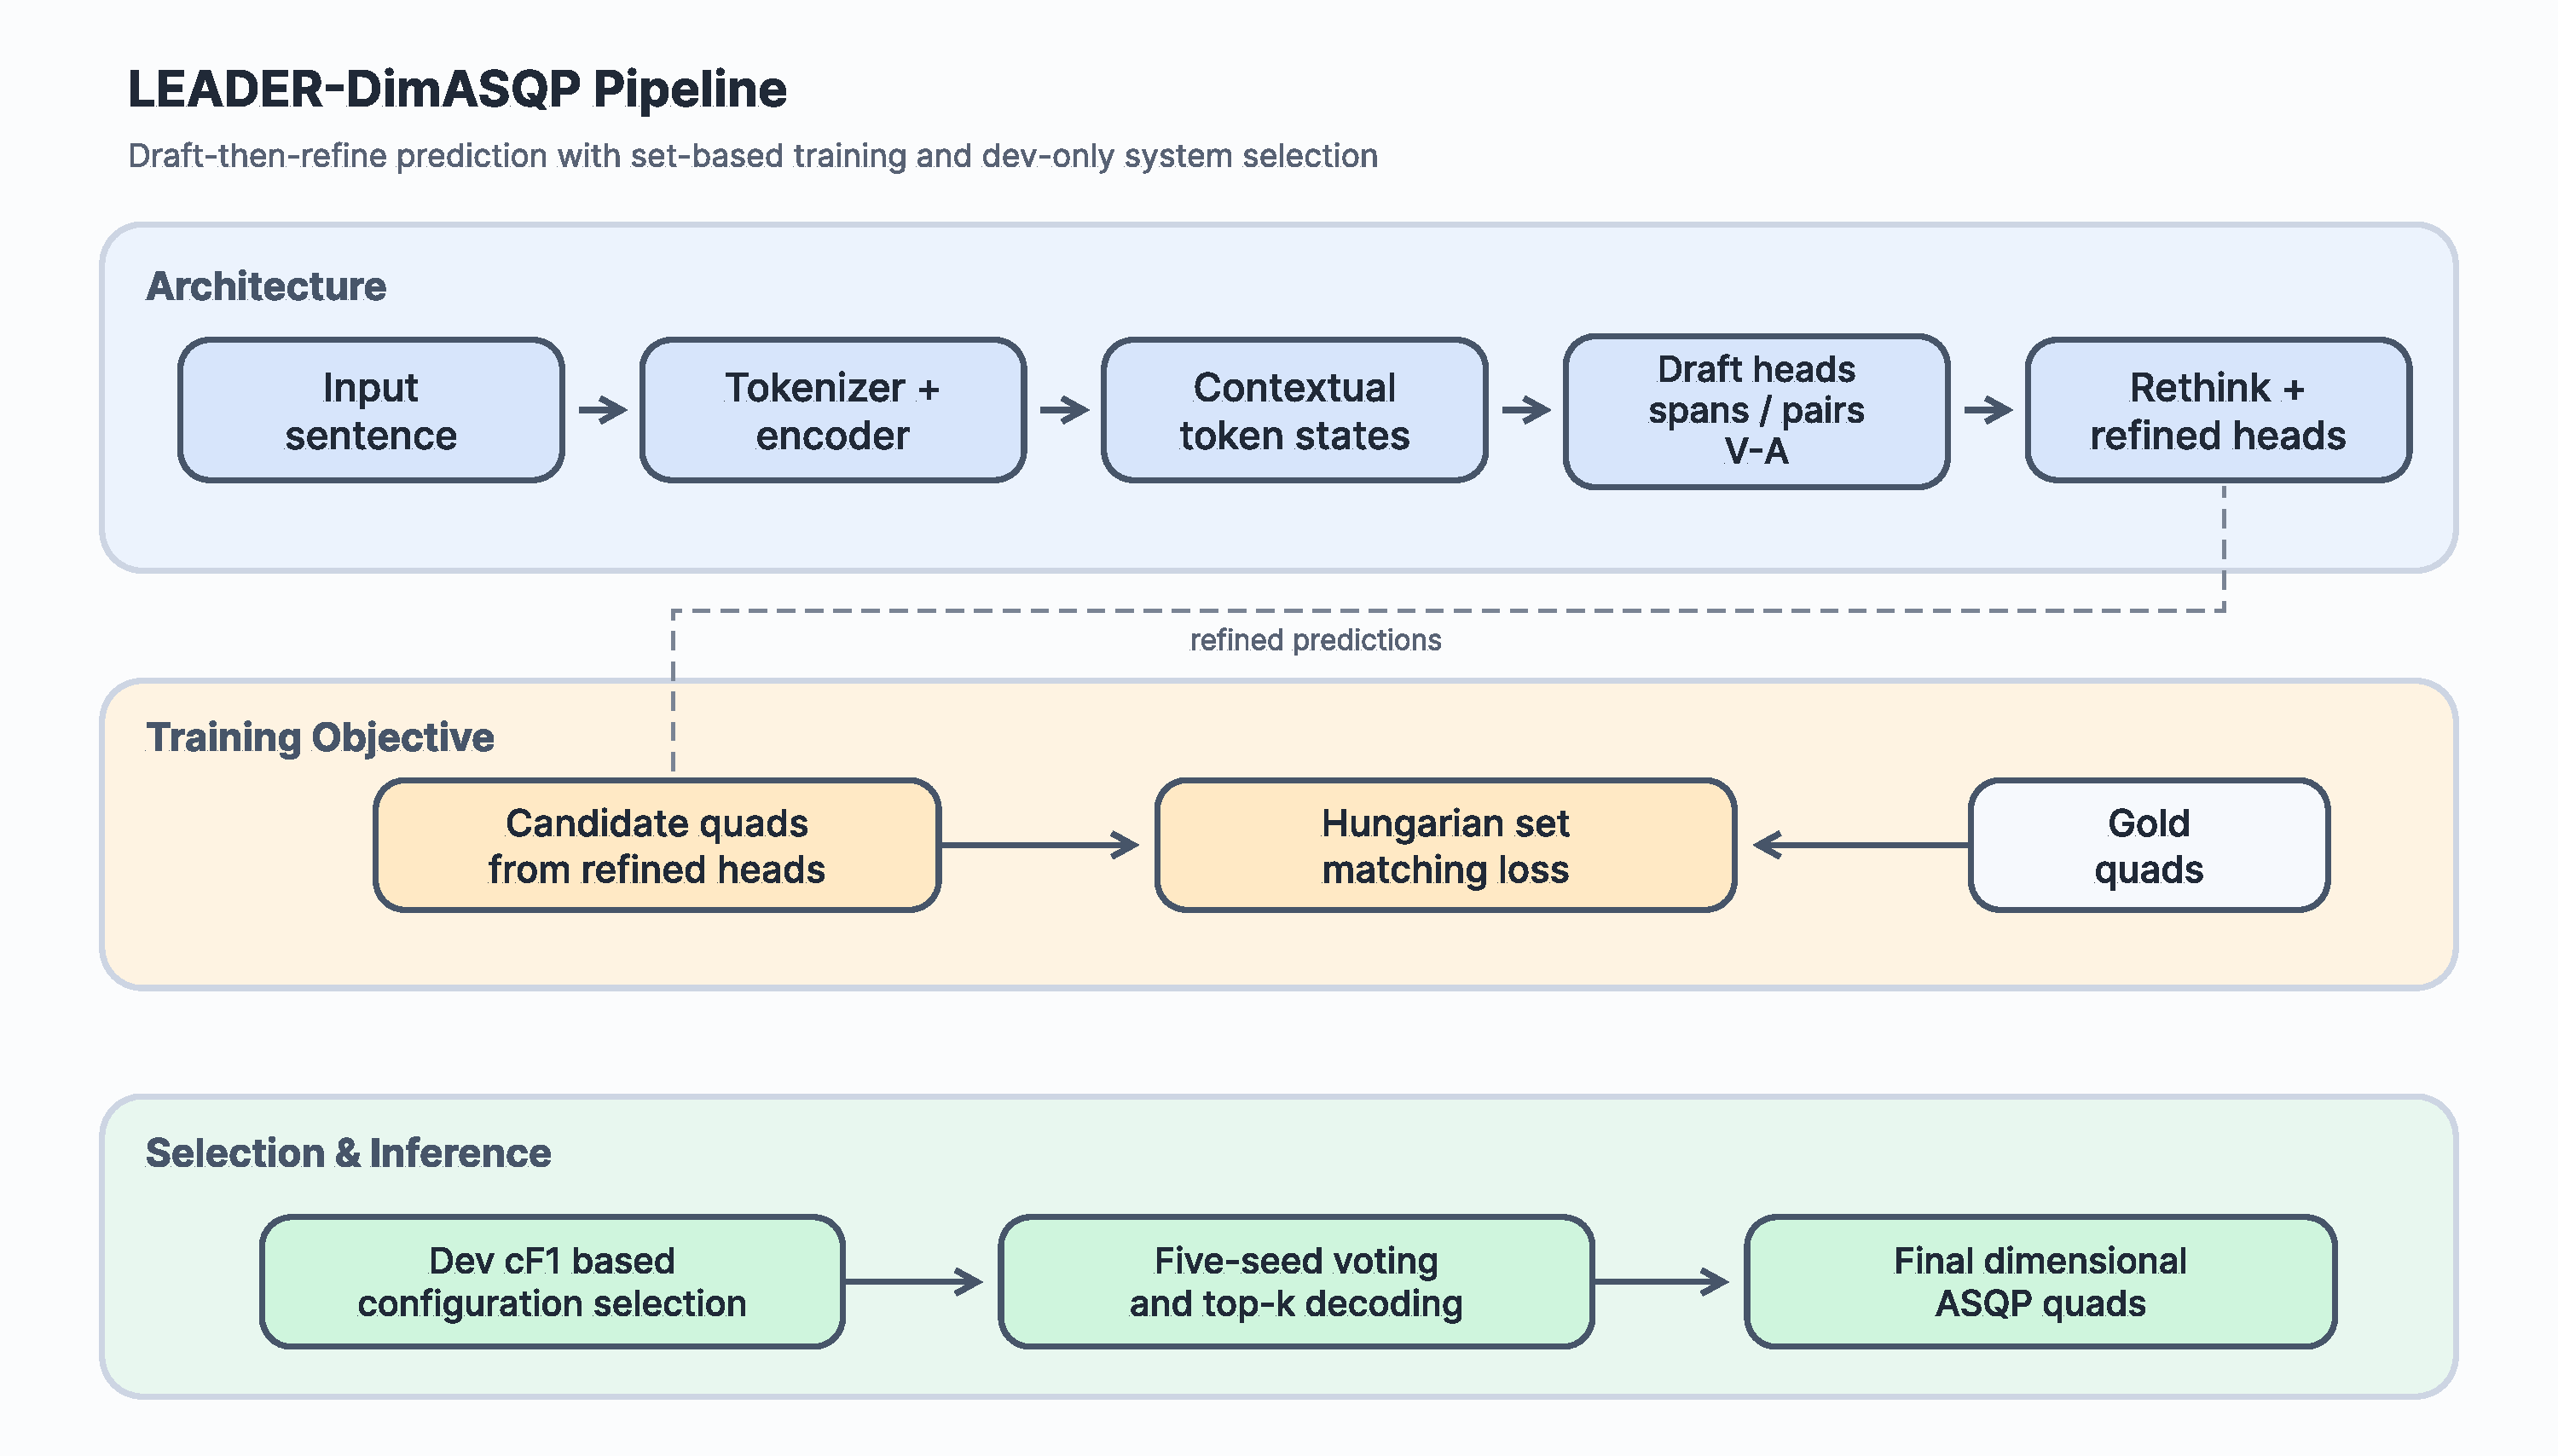
\includegraphics[width=\linewidth]{leader_pipeline.pdf}
\caption{Overview of LEADER-DimASQP. Draft span, pair, category, and
Valence--Arousal predictions are fed back into token representations
through a lightweight Rethink module. Candidate quads are optimized
with Hungarian set matching, and final predictions use dataset-specific
encoder/recipe selection with five-seed voting.}
\label{fig:pipeline}
\end{figure}

\subsection{Base Architecture with Rethink Feedback}

LEADER-DimASQP follows an extract-then-classify design. A pretrained
encoder produces contextual states $H\in\mathbb{R}^{n\times d}$. A
BIO span head predicts aspect and opinion spans. Candidate
aspect-opinion pairs are formed from decoded spans. Pair validity,
entity category, attribute category, and V--A values are predicted by
MLP heads over pooled span representations.

The core architectural component is a feature-level Rethink module. Draft
BIO, category, and V--A predictions are embedded and fused back into
the hidden states. A second set of heads then predicts from the refined
states. This gives the pair and regression heads access to soft
information about what the model has already extracted.

The BIO head predicts five labels: outside, beginning-aspect,
inside-aspect, beginning-opinion, and inside-opinion. Span boundaries
are decoded greedily in the base version. Aspect and opinion span
representations are computed by mean pooling over their token states.
For a candidate pair, the two span representations, their element-wise
product, and a distance feature are concatenated and passed to the
pair and category heads. The V--A head uses a sigmoid projection scaled
to $[1,9]$ so that predictions always fall inside the valid annotation
range.

The Rethink module is intentionally lightweight. It does not call the
encoder a second time. Instead, it maps draft labels into learned
embeddings and combines them with the original contextual states. This
design keeps inference cost lower than a full cascade while allowing
the second-stage heads to condition on draft structure. In later
ablations, this component remains positive but its marginal gain becomes
smaller when large encoders and five-seed ensembles are used.

\subsection{Hungarian Matching}

Candidate pair enumeration produces more predictions than gold quads.
Directly aligning predictions and gold quads by order is unstable.
We therefore build a cost matrix between candidates and gold quads and
solve the assignment with the Hungarian algorithm~\cite{kuhn1955hungarian}. The cost combines
span overlap, entity loss, attribute loss, pair validity, and V--A
Huber distance. The final loss is a weighted sum of BIO loss, pair
loss, entity loss, attribute loss, V--A loss, and a consistency term
between draft and refined predictions.

This assignment step is important because candidate enumeration creates
a Cartesian product of spans. Without matching, the training objective
implicitly assumes that generated candidates and gold quads are in the
same order. That assumption is false as soon as a sentence has more
than one aspect or opinion. Hungarian matching turns the prediction
problem into a set prediction problem and gives each gold quad the
closest candidate under the task-relevant cost, following the broader
set-prediction idea used in DETR~\cite{carion2020detr}.

\subsection{Training Stabilization}

We use three practical stabilizers: mild FGM adversarial training
($\epsilon=0.1$), exponential moving average with decay $0.999$, and
top-$k$ checkpoint saving. Early experiments showed that strong FGM
($\epsilon=0.5$) destabilized training, while mild perturbation~\cite{miyato2017adv} and
EMA gave more reliable validation cF1.

\subsection{Data Augmentation and Transfer}

The augmentation setting uses back-translation~\cite{sennrich2016bt} to enlarge the training data. For English,
we translate through German, French, Chinese, and Russian pivots. For
non-English data, language-specific pivots are used when available.
Span annotations are kept only when aspect and opinion substrings can
be relocated in the augmented sentence.

The cross-lingual transfer setting uses the best Chinese restaurant
checkpoint as a source model for low-resource target languages. This
checkpoint is chosen because Chinese restaurant is the largest
restaurant dataset and gave the strongest source validation score in
our logs. This is particularly useful for Russian, Tatar, and Ukrainian restaurant data. Japanese
additionally uses MeCab-based span trimming~\cite{kudo2004mecab} to remove trailing particles
and auxiliary tokens from predicted spans.

\subsection{Paraphrase Filtering}

For Japanese and later for several non-English languages, we tested
label-preserving paraphrase augmentation. A DeepSeek paraphrase is
accepted only when gold aspect and opinion strings remain present.
COMET scores~\cite{rei2022comet} are then used as a quality filter. Japanese improves as
the threshold rises from 0.92 to 0.96, but degrades at 0.965, showing
a quality--quantity sweet spot. Ukrainian improves only when
back-translation and paraphrase data are combined rather than replacing
one with the other.

\subsection{Encoder Selection and Ensemble}

The encoder-scaling setting replaces mDeBERTa with XLM-R-large for selected languages. This
substantially improves Russian, Tatar, and Japanese ensemble results.
The language-specific encoder setting then tests language-specific encoders. Japanese uses
\path{ku-nlp/deberta-v2-large-japanese}; Chinese laptop uses
\path{hfl/chinese-roberta-wwm-ext-large}; Russian tests
\path{ai-forever/ruRoberta-large}. Language-specific encoders are
highly beneficial for Japanese and Chinese laptop data, but Russian
performs better with XLM-R-large. This selection is made only on
development data; hidden-test labels are not used.

All final systems use five seeds. At inference time, quads are kept
when enough seeds agree on the categorical triple. Some datasets also
use top-$k$ span decoding, which keeps near-boundary BIO alternatives
to improve recall.

\subsection{Implementation Details}

Table~\ref{tab:impl} summarizes the main implementation settings. We
use the same training code for all datasets and change only the data,
encoder, augmentation source, and inference thresholds. This was
important for fair ablations: most configuration changes alter exactly one
factor, such as the encoder or COMET threshold. All hyperparameters
below are selected on development data; hidden-test labels are never
used for model or threshold selection.

\begin{table}[!h]
\centering
\caption{Core implementation settings.}
\label{tab:impl}
\footnotesize
\begin{tabular}{p{0.31\linewidth}p{0.61\linewidth}}
\toprule
Item & Setting \\
\midrule
Seeds & 42, 123, 456, 789, 1024 \\
Training epochs & up to 30 with validation-based selection \\
Early stopping & patience 8 on development cF1 \\
Batch size & 8 for base-size encoders; 4 with gradient accumulation 2 for large encoders \\
Maximum sequence length & 256 wordpiece tokens \\
Optimizer & AdamW with linear warmup and decay \\
Warmup ratio & 0.1 of optimizer update steps \\
Weight decay / clipping & 0.01 weight decay, 1.0 max gradient norm \\
Base encoder learning rate & $1.5\times 10^{-5}$ in stable base-model runs \\
Head learning rate & $7.5\times 10^{-5}$ in stable base-model runs \\
FGM epsilon & 0.1 \\
EMA decay & 0.999 \\
Main loss weights & span 2.0, pair 1.0, entity 1.0, attribute 1.0 \\
Checkpoints & top-3 validation checkpoints per seed \\
Final inference & five-seed voting with dataset-specific vote/top-$k$ \\
Hardware & single NVIDIA RTX 3090/4090-class GPU with 24GB memory \\
Training time & roughly 30--40 minutes per 30-epoch seed for base-size runs; large-encoder runs vary by dataset \\
\bottomrule
\end{tabular}
\end{table}

\section{Experimental Setup}

\subsection{Datasets}

Table~\ref{tab:data} lists the eight development datasets used in our
experiments. The training sizes show the strong imbalance across
language-domain pairs, from 1,240 sentences for the smallest
low-resource restaurant datasets to 6,050 sentences for Chinese
restaurant.

\begin{table}[!h]
\centering
\caption{Datasets in Track~A Subtask~3.}
\label{tab:data}
\footnotesize
\begin{tabular}{lllrl}
\toprule
Dataset & Language & Domain & Train sent. & Main challenge \\
\midrule
eng\_restaurant & English & restaurant & 2,284 & high precision extraction \\
eng\_laptop & English & laptop & 4,076 & many entity and attribute labels \\
jpn\_hotel & Japanese & hotel & 1,600 & span boundaries and morphology \\
rus\_restaurant & Russian & restaurant & 1,240 & low-resource transfer \\
tat\_restaurant & Tatar & restaurant & 1,240 & low-resource language \\
ukr\_restaurant & Ukrainian & restaurant & 1,240 & low-resource transfer \\
zho\_restaurant & Chinese & restaurant & 6,050 & large source dataset \\
zho\_laptop & Chinese & laptop & 3,490 & domain and label diversity \\
\bottomrule
\end{tabular}
\end{table}

\subsection{Baselines and External Systems}

We compare to the official baselines reported in the DimABSA dataset
paper: Llama-3.3 70B, GPT-OSS 120B, GPT-5 mini zero-shot, and Kimi K2
zero-shot. We also report representative development-set scores from
the SemEval-2026 Task~3 overview paper, including PALI, Takoyaki, PAI,
NYCU, ALPS-Lab, and AILS-NTUA~\cite{overview2026,ailsntua2026}. Because our numbers are development-set
results from the current codebase, all external comparisons should be
read as reference comparisons rather than final hidden-test claims.

\subsection{Configuration Naming}

For reproducibility, we keep the project log identifiers in
parentheses, but the paper refers to configurations by their main
methodological change. The stable Rethink base model (V3) combines
Hungarian matching, mild FGM, EMA, and span-loss reweighting. The
augmentation setting (V5) adds back-translation and dual-layer
ensembling. The cross-lingual transfer setting (V6) adds transfer from
the Chinese restaurant source model and Japanese MeCab post-processing.
The paraphrase-filtered settings (V13 variants) tune COMET thresholds
and language-specific augmentation recipes. The encoder-scaling setting
(V15) uses XLM-R-large for selected languages, and the language-specific
encoder setting (V16) tests language-specific pretrained encoders. The
final system chooses the best validated configuration for each dataset.

\section{Results}

\subsection{Configuration Evolution}

Table~\ref{tab:versions} summarizes the main configuration progression.
The augmented ensemble is the first full-language augmented setting.
Cross-lingual transfer and Japanese post-processing close much of the
gap for low-resource languages. The paraphrase-filtered settings show
that augmentation must be selected by language and data quality. The
encoder-scaling and language-specific encoder settings show that
encoder choice can dominate earlier data-level changes. A dash denotes
that the configuration was not evaluated or not used for that dataset.
If a configuration does not modify a dataset, we carry forward the
previous validated score for that dataset when computing the
eight-dataset mean.

\begin{table}[t]
\centering
\caption{Validated development cF1 after each main configuration
stage. When a stage does not change a dataset, the previous validated
score is carried forward; ``--'' denotes not evaluated or not used.}
\label{tab:versions}
\resizebox{\textwidth}{!}{
\begin{tabular}{lccccccccc}
\toprule
Configuration & Eng-R & Eng-L & Jpn-H & Rus-R & Tat-R & Ukr-R & Zho-R & Zho-L & Mean \\
\midrule
Augmented ensemble (V5) & 0.6554 & 0.3304 & 0.2660 & 0.3633 & 0.3979 & 0.3984 & 0.4745 & 0.3554 & 0.4052 \\
Cross-lingual transfer (V6) & 0.6554 & 0.3304 & 0.3312 & 0.4520 & 0.4538 & 0.4674 & 0.4745 & 0.3526 & 0.4397 \\
Paraphrase-filtered recipes (V13) & -- & -- & 0.3765 & 0.4724 & 0.4538 & 0.5068 & -- & 0.3791 & -- \\
Encoder scaling (V15) & -- & -- & 0.3962 & 0.5267 & 0.4821 & 0.4957 & -- & 0.3904 & -- \\
Language-specific encoders (V16) & 0.6949 & 0.3035 & 0.4500 & 0.5152 & -- & -- & 0.5669 & 0.4487 & -- \\
\textbf{Best validated} & \textbf{0.6949} & \textbf{0.3304} & \textbf{0.4500} & \textbf{0.5267} & \textbf{0.4821} & \textbf{0.5068} & \textbf{0.5669} & \textbf{0.4487} & \textbf{0.5008} \\
\bottomrule
\end{tabular}}
\end{table}

The best validated system improves over the cross-lingual transfer
baseline by 6.11 points on average. The largest gains come from Japanese hotel (+11.88 points), Chinese
restaurant (+9.24), Russian restaurant (+7.47), and Chinese laptop
(+9.61). English laptop is the only dataset where the language-specific
encoder setting is below the cross-lingual transfer setting, so the best
validated system selects the transfer result for that dataset. This confirms that the
laptop domain remains difficult even with a stronger encoder. All
configuration and threshold choices in this selection are based only on
development cF1; hidden-test labels are never used.

The progression also shows why reporting only the latest configuration
is misleading. The augmented ensemble is already strong for English
restaurant and Chinese restaurant, but weak for Japanese and the
low-resource Slavic/Turkic datasets. Cross-lingual transfer fixes most
of this gap. Paraphrase-filtered recipes then show that augmentation is
not globally useful: it improves Japanese, Russian, Ukrainian, and
Chinese laptop under different recipes, but does not improve Tatar.
Encoder scaling and language-specific tokenization can dominate all
earlier data-level changes.

This progression suggests that multilingual DimASQP is not governed by
a single bottleneck. Japanese and Chinese laptop mainly benefit from
tokenizer and pretraining match, Russian and Tatar benefit more from
multilingual transfer and encoder scale, while Ukrainian depends on
augmentation diversity. This explains why a best validated
per-dataset selection outperforms a universal recipe.

\subsection{Comparison with Official Development-Set Baselines}

Table~\ref{tab:baseline} compares the best validated system with
official development-set baselines from the DimABSA dataset paper. Our
best validated system is higher than the strongest official baseline on
all eight development datasets. The mean gain over Llama-3.3 70B, the
strongest official baseline by average cF1, is 11.46 points.

\begin{table}[t]
\centering
\caption{Comparison with official development-set baselines from arXiv:2601.23022.}
\label{tab:baseline}
\resizebox{\textwidth}{!}{
\begin{tabular}{lccccccccc}
\toprule
System & Eng-R & Eng-L & Jpn-H & Rus-R & Tat-R & Ukr-R & Zho-R & Zho-L & Mean \\
\midrule
Llama-3.3 70B & 0.5048 & 0.2483 & 0.3577 & 0.4118 & 0.3702 & 0.4070 & 0.4391 & 0.3506 & 0.3862 \\
GPT-OSS 120B & 0.5013 & 0.2411 & 0.4151 & 0.3683 & 0.3094 & 0.3663 & 0.4249 & 0.3551 & 0.3727 \\
GPT-5 mini 0-shot & 0.4036 & 0.2304 & 0.0907 & 0.2508 & 0.1974 & 0.2465 & 0.2481 & 0.1356 & 0.2254 \\
Kimi K2 0-shot & 0.3740 & 0.2805 & 0.1309 & 0.2656 & 0.2310 & 0.2974 & 0.2975 & 0.1569 & 0.2542 \\
\textbf{Best validated} & \textbf{0.6949} & \textbf{0.3304} & \textbf{0.4500} & \textbf{0.5267} & \textbf{0.4821} & \textbf{0.5068} & \textbf{0.5669} & \textbf{0.4487} & \textbf{0.5008} \\
\bottomrule
\end{tabular}}
\end{table}

\subsection{Comparison with Reported Shared-Task Systems}

Table~\ref{tab:systems} compares against representative reported
shared-task systems. The best validated system is competitive with the best
reported systems and exceeds the reported development-set top score on
Japanese hotel, Tatar restaurant, and Chinese restaurant.
It remains below the best reported scores on English laptop, Russian,
Ukrainian, and Chinese laptop.

The comparison suggests different failure modes. English laptop and
Chinese laptop both have richer entity-attribute inventories than
restaurant data, so category errors are more frequent. Russian and
Ukrainian benefit from transfer and ensembling, but the best reported
systems still appear to have stronger language-specific adaptation.
Japanese and Tatar, in contrast, benefit strongly from our final
encoder and ensemble choices.

\begin{table}[t]
\centering
\caption{Comparison with representative reported systems from the shared-task overview.}
\label{tab:systems}
\resizebox{\textwidth}{!}{
\begin{tabular}{lccccccccc}
\toprule
System & Eng-R & Eng-L & Jpn-H & Rus-R & Tat-R & Ukr-R & Zho-R & Zho-L & Mean \\
\midrule
PALI & 0.6395 & 0.3793 & 0.4252 & 0.5496 & 0.4443 & 0.5307 & 0.5357 & 0.4319 & 0.4920 \\
PAI & -- & 0.3758 & -- & \textbf{0.5599} & 0.4523 & \textbf{0.5437} & 0.5360 & 0.4316 & -- \\
NYCU & -- & -- & -- & -- & -- & -- & 0.5521 & \textbf{0.4824} & -- \\
Takoyaki & 0.6514 & \textbf{0.4227} & 0.4086 & 0.5130 & 0.4736 & 0.5019 & 0.4966 & 0.3745 & 0.4803 \\
ALPS-Lab & 0.6202 & 0.3395 & 0.3617 & 0.5042 & 0.4404 & 0.5163 & 0.4853 & 0.3968 & 0.4581 \\
AILS-NTUA & 0.5988 & 0.2694 & 0.3747 & 0.4369 & 0.3306 & 0.4154 & 0.4544 & 0.3703 & 0.4063 \\
Shared-task avg. & 0.5398 & 0.2908 & 0.3259 & 0.4526 & 0.3581 & 0.4446 & 0.4728 & 0.3602 & 0.4056 \\
\textbf{Best validated} & \textbf{0.6949} & 0.3304 & \textbf{0.4500} & 0.5267 & \textbf{0.4821} & 0.5068 & \textbf{0.5669} & 0.4487 & \textbf{0.5008} \\
\bottomrule
\end{tabular}}
\end{table}

\section{Ablation Studies}

\subsection{Five-Seed Ensemble}

Table~\ref{tab:ensemble} shows that five-seed ensembling gives a
consistent gain on all eight datasets. The average improvement over
the five-seed mean is 4.76 points. This is the most reliable
method-level contribution in the final system. Its ensemble mean
differs slightly from the best validated mean in
Table~\ref{tab:versions} because the latter additionally chooses the
best development-set recipe for each dataset; for English laptop, it
selects the cross-lingual transfer result rather than the
language-specific encoder ensemble result.

\begin{table}[t]
\centering
\caption{Contribution of five-seed ensembling.}
\label{tab:ensemble}
\begin{tabular}{lcccc}
\toprule
Dataset & Best seed & Seed mean & Ensemble & Gain \\
\midrule
jpn\_hotel & 0.4128 & 0.4026 & 0.4466 & +4.40 \\
rus\_restaurant & 0.4817 & 0.4699 & 0.5267 & +5.68 \\
zho\_laptop & 0.4010 & 0.3940 & 0.4487 & +5.47 \\
ukr\_restaurant & 0.4736 & 0.4541 & 0.5068 & +5.27 \\
tat\_restaurant & 0.4282 & 0.4047 & 0.4821 & +7.74 \\
eng\_restaurant & 0.6759 & 0.6728 & 0.6949 & +2.21 \\
eng\_laptop & 0.2943 & 0.2892 & 0.3035 & +1.43 \\
zho\_restaurant & 0.5234 & 0.5083 & 0.5669 & +5.86 \\
\midrule
\textbf{Mean} & 0.4614 & 0.4495 & 0.4970 & \textbf{+4.76} \\
\bottomrule
\end{tabular}
\end{table}

\subsection{Language-Specific Encoders}

Language-specific encoders are not uniformly better. Japanese improves
from 0.3962 with XLM-R-large to 0.4500 with Japanese DeBERTa, and
Chinese laptop improves from 0.3904 to 0.4487 with Chinese RoBERTa.
Russian drops from 0.5267 with XLM-R-large to 0.5152 with
ruRoberta-large. This suggests that language-specific pretraining must
be validated empirically rather than assumed to dominate multilingual
pretraining.

The contrast between Japanese/Chinese and Russian is important.
Language-specific encoders help when their tokenizer and pretraining
corpus better preserve task-relevant boundaries and domain-specific
categories. However, they can underperform when they lose the
cross-lingual regularization and transfer ability of XLM-R-large. Thus,
encoder selection must be validated empirically rather than chosen by
language identity alone.

\subsection{Rethink and Augmentation at Large Scale}

Early mDeBERTa-base experiments showed large gains from the Rethink
module and data augmentation. Thus, Rethink is best viewed as the
architecture-level contribution that builds a strong single-model
baseline. In the final language-specific encoder setting, however, its marginal gain shrinks:
on English restaurant with DeBERTa-v3-large, Rethink improves ensemble
cF1 from 0.6913 to 0.6949. On Japanese with language-specific DeBERTa and
five-seed ensembling, paraphrase augmentation slightly hurts the
ensemble result, 0.4466 with augmentation versus 0.4500 without
augmentation. These results suggest that structural refinement,
synthetic-data regularization, encoder capacity, and ensembling can
partly substitute for one another.

This result does not mean that Rethink is unnecessary. Instead, Rethink
provides explicit task-structure feedback, which is most useful when
encoder representations are less specialized. With large encoders and
five-seed voting, part of the same benefit is absorbed by representation
capacity and ensemble stability.

\subsection{Language-Specific Augmentation Recipes}

Table~\ref{tab:recipes} shows the final augmentation decision for the
five non-English non-Chinese-restaurant datasets that required the
most tuning. The main lesson is that the best recipe depends on both
the baseline strength and the quality of generated data. Japanese
benefits from high-threshold paraphrase filtering when using mDeBERTa,
but the final language-specific Japanese encoder works best without paraphrase
augmentation. Ukrainian requires combining back-translation and
paraphrase, while Tatar does not benefit from the paraphrase recipe.

\begin{table}[t]
\centering
\caption{Language-specific augmentation and encoder decisions.}
\label{tab:recipes}
\begin{tabular}{llll}
\toprule
Dataset & Best configuration & Main decision & dev cF1 \\
\midrule
jpn\_hotel & Lang.-specific encoder & Japanese DeBERTa, no paraphrase & 0.4500 \\
rus\_restaurant & Encoder scaling & XLM-R-large, vote/top-$k$ sweep & 0.5267 \\
tat\_restaurant & Encoder scaling & XLM-R-large, no paraphrase gain & 0.4821 \\
ukr\_restaurant & Paraphrase-filtered recipe & BT plus paraphrase with mDeBERTa & 0.5068 \\
zho\_laptop & Lang.-specific encoder & Chinese RoBERTa large, topk=0.10 & 0.4487 \\
\bottomrule
\end{tabular}
\end{table}

\section{Negative Results and Discussion}

\paragraph{CRF decoding.}
Adding a linear-chain CRF~\cite{lafferty2001crf} and \textsc{NULL} anchors did not improve
over the stable Rethink base model. The best CRF setting reached 0.6249
on English restaurant, below the base score of 0.6278. The likely reason is that BIO constraints
are simple, while CRF transition parameters overfit the small training
set.

\paragraph{Over-filtering paraphrases.}
COMET filtering improves Japanese paraphrase quality up to a point.
The cF1 rises from 0.3317 at threshold 0.92 to 0.3565 at 0.96, then
drops to 0.3418 at 0.965. Data quality matters, but too much filtering
causes underfitting.

\paragraph{Cross-encoder and LLM fusion.}
Combining paraphrase-filtered and encoder-scaled checkpoints through a
10-seed cross-encoder ensemble reduces Japanese cF1 from 0.3962 to
0.3721. Adding DeepSeek
candidate quads also hurts: the best smart fusion remains below the
encoder-scaled top-$k$ baseline. LLM candidates improve recall but introduce too
many category and span false positives, despite related systems showing
that encoder and LLM predictions can be complementary in other DimABSA
settings~\cite{quadai2026}.

\paragraph{Confidence weighting and uncertainty weighting.}
Confidence-weighted ensemble voting lowers the eight-dataset mean from
0.5008 to 0.4901. Uncertainty-weighted multi-task loss is unstable:
it slightly helps English restaurant but sharply hurts Japanese. Fixed
loss weights remain more robust. This contrasts with LogSigma, where
uncertainty weighting is effective for related DimABSA regression
settings~\cite{logsigma2026}.

Taken together, these negative results show that additional model
complexity is not automatically beneficial for DimASQP. Because cF1
requires exact categorical matching before V--A credit is assigned,
recall-oriented fusion methods can easily introduce span or category
false positives that outweigh their gains.

\section{Error Analysis}

The remaining errors fall into four broad groups. First, span boundary
errors are still common, especially in Japanese and laptop reviews
where aspect terms are short or embedded in longer noun phrases.
Second, category confusion remains difficult in domains with many
entity-attribute combinations, especially English and Chinese laptop.
Third, low-resource languages still suffer from false negatives even
after transfer and ensembling. Fourth, extreme V--A values are often
regressed toward the middle of the scale, reducing cF1 even when the
categorical quad is correct.

These errors explain why the final system is strong on Japanese hotel,
Tatar restaurant, and Chinese restaurant, but still behind the best
reported systems on English laptop, Russian, Ukrainian, and Chinese
laptop. Future work should focus on category-aware decoding, better
domain adaptation for laptop data, and calibrated V--A distributions
rather than point regression alone.

The dominant error type also differs by dataset. For Japanese, many
remaining errors involve boundary over-expansion, where a predicted
opinion span includes particles or auxiliary words. For laptop data,
errors more often involve assigning a correct span to a wrong
entity-attribute category, suggesting that category-aware decoding may
be more useful than further span refinement.

\section{Limitations}

There are three limitations. First, the final system is a mixture of
dataset-specific choices. This is effective for a shared task and is
chosen only with development data, but it is less elegant than a single
universal multilingual model. Second, all comparisons in this draft use
development-set results from the current project logs and external
reported scores. Final hidden-test evaluation may change the ranking.
Third, the system still uses exact or near-exact span matching
assumptions during augmentation.
This keeps labels reliable, but it rejects paraphrases that would be
semantically valid if span alignment were solved with a stronger
alignment model.

Despite these limitations, the configuration study is useful because it
separates robust improvements from attractive but unreliable ones.
Five-seed ensembling, validated encoder selection, and task-aware
augmentation survive repeated tests. LLM fusion, confidence-weighted
voting, and automatic uncertainty-weighted losses do not yet provide
reliable gains for this setting.

\section{Conclusion}

We presented \textbf{LEADER-DimASQP}, a complete multilingual system
for SemEval-2026 Task~3 Track~A Subtask~3. The system first establishes
a strong DimASQP architecture with lightweight Rethink feedback and
Hungarian set matching. The broader lesson is that the best final
system is not a single universal recipe: after the base model is
stabilized, performance depends on selecting the right encoder,
augmentation policy, and inference threshold for each dataset. The
best validated per-dataset system reaches 0.5008 mean development cF1, exceeds
the official DimABSA development-set baselines on all eight datasets,
and is competitive with strong reported shared-task systems. The most
robust final gains come from five-seed ensembling and validated
language-specific encoder selection, while Rethink remains a useful
architecture-level component whose marginal gain decreases with large
encoders and ensembles.

\begin{thebibliography}{99}\small

\bibitem{cai2021acos}
Cai, H., Xia, R., Yu, J.:
Aspect-category-opinion-sentiment quadruple extraction with implicit
aspects and opinions. In: Proc. of ACL-IJCNLP (2021)

\bibitem{zhang2021asqp}
Zhang, W., Li, X., Deng, Y., Bing, L., Lam, W.:
Aspect sentiment quad prediction as paraphrase generation. In: Proc.
of EMNLP (2021)

\bibitem{carion2020detr}
Carion, N., Massa, F., Synnaeve, G., Usunier, N., Kirillov, A.,
Zagoruyko, S.:
End-to-end object detection with transformers. In: Proc. of ECCV
(2020)

\bibitem{dimabsa2026}
Lee, L.-H., Yu, L.-C., Loukashevich, N., Alimova, I., Panchenko, A.,
Lin, T.-M., Xu, Z.-Y., Zhou, J.-Y., Zheng, G., Wang, J.,
Awasthi, S., Becker, J., Wahle, J.P., Ruas, T., Muhammad, S.H.,
Mohammad, S.M.:
DimABSA: Building multilingual and multidomain datasets for dimensional
aspect-based sentiment analysis. arXiv:2601.23022 (2026)

\bibitem{overview2026}
Yu, L.-C., Becker, J., Muhammad, S.H., Abdulmumin, I., Lee, L.-H.,
Lin, Y.-L., Wang, J., Wahle, J.P., Ruas, T., Loukachevitch, N.,
Panchenko, A., Alimova, I., Wanzare, L., Odhiambo, N., Gipp, B.,
Chang, K.-W., Mohammad, S.M.:
SemEval-2026 Task 3: Dimensional aspect-based sentiment analysis
(DimABSA). arXiv:2604.07066 (2026)

\bibitem{he2023deberta}
He, P., Gao, J., Chen, W.:
DeBERTaV3: Improving DeBERTa using ELECTRA-style pre-training with
gradient-disentangled embedding sharing. In: Proc. of ICLR (2023)

\bibitem{kuhn1955hungarian}
Kuhn, H.W.:
The Hungarian method for the assignment problem. Naval Research
Logistics Quarterly 2(1-2), 83-97 (1955)

\bibitem{kudo2004mecab}
Kudo, T., Yamamoto, K., Matsumoto, Y.:
Applying conditional random fields to Japanese morphological analysis.
In: Proc. of EMNLP, pp. 230--237 (2004)

\bibitem{lafferty2001crf}
Lafferty, J., McCallum, A., Pereira, F.:
Conditional random fields: Probabilistic models for segmenting and
labeling sequence data. In: Proc. of ICML (2001)

\bibitem{liu2019roberta}
Liu, Y., Ott, M., Goyal, N., Du, J., Joshi, M., Chen, D., Levy, O.,
Lewis, M., Zettlemoyer, L., Stoyanov, V.:
RoBERTa: A robustly optimized BERT pretraining approach.
arXiv:1907.11692 (2019)

\bibitem{conneau2020xlmr}
Conneau, A., Khandelwal, K., Goyal, N., Chaudhary, V., Wenzek, G.,
Guzman, F., Grave, E., Ott, M., Zettlemoyer, L., Stoyanov, V.:
Unsupervised cross-lingual representation learning at scale. In: Proc.
of ACL (2020)

\bibitem{miyato2017adv}
Miyato, T., Dai, A.M., Goodfellow, I.:
Adversarial training methods for semi-supervised text classification.
In: Proc. of ICLR (2017)

\bibitem{rei2022comet}
Rei, R., Treviso, M., Guerreiro, N.M., Zerva, C., Farinha, A.C.,
Maroti, C., de Souza, J.G.C., Glushkova, T., Alves, D., Lavie, A.,
Martins, A.F.T.:
CometKiwi: IST-unbabel 2022 submission for the quality estimation
shared task. In: Proc. of WMT (2022)

\bibitem{russell1980circumplex}
Russell, J.A.:
A circumplex model of affect. Journal of Personality and Social
Psychology 39(6), 1161-1178 (1980)

\bibitem{sennrich2016bt}
Sennrich, R., Haddow, B., Birch, A.:
Improving neural machine translation models with monolingual data. In:
Proc. of ACL (2016)

\bibitem{ailsntua2026}
Gazetas, S., Filandrianos, G., Lymperaiou, M., Tzouveli, P.,
Voulodimos, A., Stamou, G.:
AILS-NTUA at SemEval-2026 Task 3: Efficient dimensional
aspect-based sentiment analysis.
arXiv:2603.04933 (2026)

\bibitem{quadai2026}
de Vink, A.J.W., Ventirozos, F.K., Amat-Lefort, N., Han, L.:
QuadAI at SemEval-2026 Task 3: Ensemble learning of hybrid RoBERTa and
LLMs for dimensional aspect-based sentiment analysis.
arXiv:2603.07766 (2026)

\bibitem{logsigma2026}
Hikal, B., Becker, J., Gipp, B.:
LogSigma at SemEval-2026 Task 3: Uncertainty-weighted multitask
learning for dimensional aspect-based sentiment analysis.
arXiv:2603.24896 (2026)

\end{thebibliography}

\end{document}
